\chapter{Use Cases}

Use Case diagrams define tasks that users will perform to achieve a certain goal when using our incubating box and 3d bioprinter system.

\section{The Box}

\begin{figure}[H]
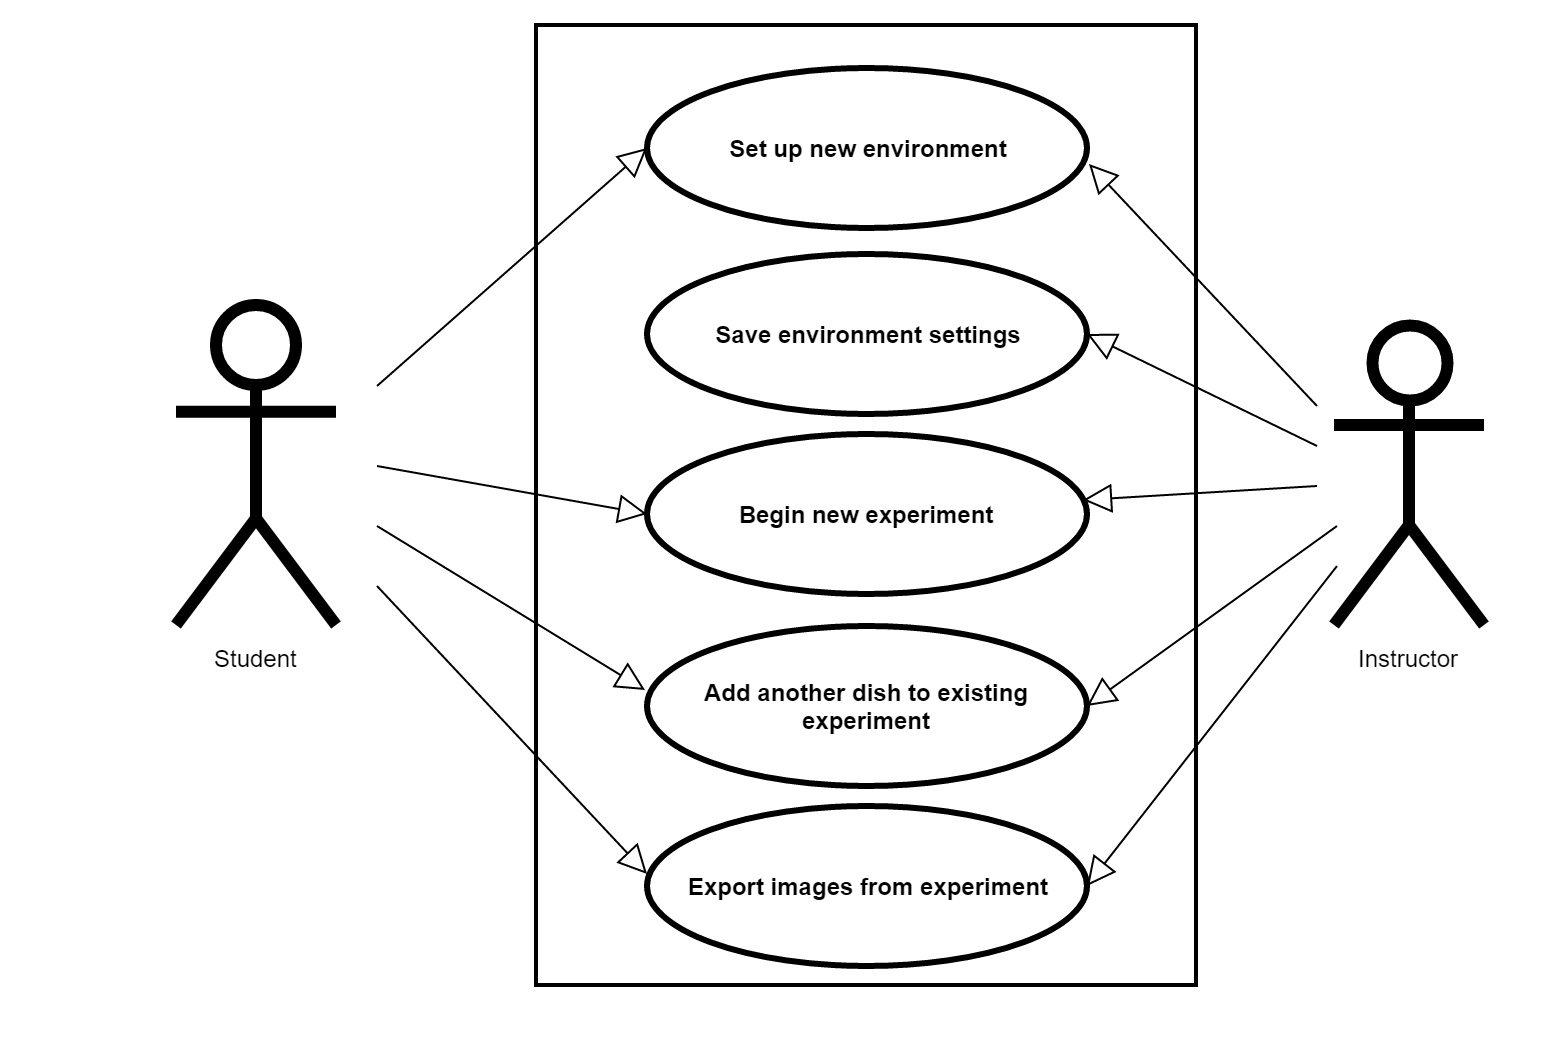
\includegraphics[scale=0.7]{box-use-case}
\caption{\label{figure:box-use-case} Use Case Diagram for The Box}
\end{figure}

\begin{enumerate}
	\item 
	\begin{itemize}
		\item Name: Set up new environment
		\item Goal: Prepare The Box to have the proper settings for the experiment that the user wants to run
		\item Actors: Student, Instructor
		\item Pre-conditions: No other experiment is currently running
		\item Steps: Either load settings that have been previously saved, or enter custom light, temperature, and image capture settings. 
		\item Post-conditions: The Box is at correct environment settings for the experiment.
		\item Exceptions: n/a
	\end{itemize}
	\item 
	\begin{itemize}
		\item Name: Save environment settings
		\item Goal: Save temperature, light, and image capture settings to prevent repetition in the future
		\item Actors: Instructor
		\item Pre-conditions: User has input custom temperature, light, and image capture settings
		\item Steps: User clicks `Save Custom environment' and enters an appropriate name
		\item Post-conditions: Future users will now be able to load this environment for future experiments
		\item Exceptions: n/a
	\end{itemize}
	\item 
	\begin{itemize}
		\item Name: Begin new experiment
		\item Goal: Begin timer and image capture on current incubated experiment
		\item Actors:  Student, Instructor
		\item Pre-conditions: User has entered proper environment settings, selected which petri dishes are present, and has placed petri dishes in The Box. The Box has been brought to proper temperature.
		\item Steps: Click `Begin Experiment'
		\item Post-conditions: Timer and image capture begins
		\item Exceptions: n/a
	\end{itemize}
	\item 
	\begin{itemize}
		\item Name: Add another dish to existing experiment
		\item Goal: Add another dish to a experiment that is already running 
		\item Actors:  Student, Instructor
		\item Pre-conditions: An experiment must be running in The Box
		\item Steps: User places dish in the box. Clicks on the appropriate petri dish to begin timer and image capture of new dish
		\item Post-conditions: New petri dish is added into the experiment and final end time is extended to accommodate 
		\item Exceptions: Incubator box is full
	\end{itemize}
	\item 
	\begin{itemize}
		\item Name: Export images from experiment
		\item Goal: Download images captured during the experiment of a single petri dish for analysis
		\item Actors:  Student, Instructor
		\item Pre-conditions: A USB drive has been inserted and detected
		\item Steps: Click `download images' button, Select the relevant dish, click `download'
		\item Post-conditions: Images transferred onto the USB drive
		\item Exceptions: No images to export
	\end{itemize}
\end{enumerate}

\section{Feasability Study}

\begin{figure}[H]
\caption{\label{figure:3D_Printer_UCD} Use Case Diagram for The Printer Components Affected by The Feasibility Study}
\includegraphics{3D_Printer_UCD}
\end{figure}

\begin{enumerate}
	\item 
	\begin{itemize}
	\item Name: Load GCODE
	\item Goal: Load GCODE files into printer memory for printing
	\item Actors: User
	\item Pre-conditions: User already has GCODE from converted 3D model
	\item Steps: Load media into printer controller
	\item Post-conditions: Printer has access to GCODE files for printing
	\item Exceptions: No valid GCODE file found
	\end{itemize}
	\item 
	\begin{itemize}
	\item Name: Load Filament
	\item Goal: Load printer filament into extruder
	\item Actors: User
	\item Pre-conditions: User has printing materials ready to load
	\item Steps For Biomaterials: Remove extruder syringe for biomaterial and insert new biomaterial 
	\item Steps For PLA Material: Remove old plastic filament spool,
	run script to remove old filament and prepare for new filament, then
	insert new filament into extruder module
	\item Post-conditions: Printer has filament loaded and is ready for calibration
	\item Exceptions: n/a
	\end{itemize}
	\item 
	\begin{itemize}
	\item Name: Preheat Bed
	\item Goal: Heat print bed for printing 
	\item Actors: User
	\item Pre-conditions: n/a
	\item Steps: Select option for preheating the bed
	\item Post-conditions: Bed is at optimal printing temperature
	\item Exceptions: n/a
	\end{itemize}
	\item 
	\begin{itemize}
	\item Name: Start Print
	\item Goal: Begin printing the 3D structure 
	\item Actors: User
	\item Pre-conditions: GCODE is loaded into printer memory, extruder is calibrated, and filament is loaded
	\item Steps: Select 3D object to print
	\item Post-conditions: Printer begins printing
	\item Exceptions: User stops print
	\end{itemize}
	\item 
	\begin{itemize}
	\item Name: View Print Status
	\item Goal: View information about current print job
	\item Actors: User
	\item Pre-conditions: The printer is printing
	\item Steps: Select option for viewing print status
	\item Post-conditions: Print status information is shown
	\item Exceptions: n/a
	\end{itemize}
	\item 
	\begin{itemize}
	\item Name: Stop Print
	\item Goal: Stop all printer activity
	\item Actors: User
	\item Pre-conditions: The printer is printing
	\item Steps: Select stop option
	\item Post-conditions: Printer stops all print activity
	\item Exceptions: n/a
	\end{itemize}
	\item 
	\begin{itemize}
	\item Name: Calibrate Extruder
	\item Goal: Have extruder be automatically calibrated for printing
	\item Actors: User
	\item Pre-conditions: The filament is loaded
	\item Steps: Select option for extruder calibration, select the extruder to calibrate
	\item Post-conditions: Printer extruder is calibrated
	\item Exceptions: Filament is empty
	\end{itemize}
\end{enumerate}
